\chapter{Packing Algorithms}
\label{ch:packing_algorithms}

\section{Circle Packing}
\label{sec:circle_packing}

\subsection{Overview}
Circle packing\index{circle packing} is the study of placing non-overlapping circles within a given container (like a square or another circle) or on a surface (like a mesh) such that the total area of the circles is maximized or the density is optimized. In computational geometry, it is a classic problem in both optimization and discrete geometry, with applications ranging from material science to map labeling and data visualization. The theory of circle packing was developed extensively by Stephenson~\cite{stephenson2005}, building on the foundational work of Koebe~\cite{koebe1936} and the influential exposition of Thurston~\cite{thurston1985}.

\subsection{Definitions}

\begin{definition}[Packing Density]\label{def:packing_density}
The \textbf{packing density}\index{packing density} of a configuration of $n$ circles $\{C_1, \dots, C_n\}$ in a container $\Omega$ is the ratio
\[
\delta = \frac{\sum_{i=1}^{n} \text{Area}(C_i)}{\text{Area}(\Omega)},
\]
where the areas of $C_i$ are the portions lying inside~$\Omega$.
\end{definition}

\begin{definition}[Optimal Packing]\label{def:optimal_packing}
An \textbf{optimal packing}\index{optimal packing} is a configuration that achieves the maximum possible density for a given number of circles or a given container size. For $n$ congruent circles in the plane, the problem of determining the optimal arrangement is open for most values of $n > 7$.
\end{definition}

\begin{definition}[Circle Contact Graph]\label{def:circle_contact_graph}
The \textbf{circle contact graph}\index{circle contact graph} of a packing is a graph $G = (V, E)$ where each node $v_i \in V$ corresponds to a circle $C_i$ and an edge $(v_i, v_j) \in E$ exists if and only if circles $C_i$ and $C_j$ are tangent (touching but not overlapping).
\end{definition}

\begin{definition}[Hexagonal Packing]\label{def:hexagonal_packing}
\textbf{Hexagonal packing}\index{hexagonal packing} is the densest possible packing of congruent circles in an infinite 2D plane, achieving a density of $\delta = \frac{\pi}{2\sqrt{3}} \approx 0.9069$ (approximately $90.69\%$).
\end{definition}

\subsection{Theory}
Finding the optimal packing of $n$ circles in a container is a \textbf{non-convex optimization} problem. The most common approaches are:
\begin{enumerate}
    \item \textbf{Greedy Placement}: Placing circles one by one at the best available position (e.g., using a ``front-advancing'' algorithm).
    \item \textbf{Force-Directed Layout}\index{force-directed layout}: Treating circles as repelling particles and using a physics simulation to find an equilibrium state where they are packed tightly.
    \item \textbf{Circle Packing on Surfaces}: Using \textbf{conformal mapping} and the Circle Packing Theorem to represent any planar graph as a set of tangent circles.
    \item \textbf{Vortex-based Packing}: Packing circles into a spiral or vortex to fill a circular container.
\end{enumerate}

For identical circles, the hexagonal lattice is optimal in 2D. For circles of different sizes (Apollonian gaskets), the packing can achieve $100\%$ density in the limit.

\begin{theorem}[Circle Packing Theorem]\label{thm:circle_packing_thm}
\textbf{(Koebe--Andreev--Thurston)} Every connected planar graph $G$ can be represented as the tangency graph of a circle packing in the plane (or on the sphere), and such a representation is unique up to Möbius transformations.
\end{theorem}

\begin{proof}
The proof proceeds in two stages. First, Andreev's theorem provides existence for triangulations using a discrete analogue of the Riemann mapping theorem. Second, Koebe's original result~\cite{koebe1936} establishes that every planar graph is a subgraph of a triangulation. Thurston~\cite{thurston1985} gave an influential expository account combining these ideas with conformal mapping theory. See Stephenson~\cite[Chapter~3]{stephenson2005} for a self-contained modern treatment.
\end{proof}

\begin{corollary}\label{cor:hexagonal_optimal}
The hexagonal lattice packing of congruent circles in $\mathbb{R}^2$ is optimal among all packings of congruent circles, with density $\frac{\pi}{2\sqrt{3}}$.
\end{corollary}

\begin{figure}[htbp]
\centering
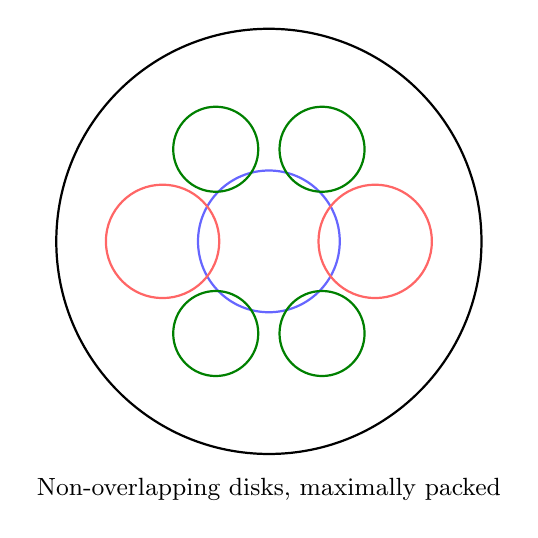
\begin{tikzpicture}[scale=0.9]
  \draw[thick] (0,0) circle (3);
  \draw[blue!60,thick] (0,0) circle (1);
  \draw[red!60,thick] (1.5,0) circle (0.8);
  \draw[red!60,thick] (-1.5,0) circle (0.8);
  \draw[green!50!black,thick] (0.75,1.3) circle (0.6);
  \draw[green!50!black,thick] (-0.75,1.3) circle (0.6);
  \draw[green!50!black,thick] (0.75,-1.3) circle (0.6);
  \draw[green!50!black,thick] (-0.75,-1.3) circle (0.6);
  \node[font=\small] at (0,-3.5) {Non-overlapping disks, maximally packed};
\end{tikzpicture}
\caption{Circle packing: placing non-overlapping disks of varying radii inside a bounding region.}
\label{fig:circle_packing}
\end{figure}


\begin{example}[Greedy Packing Trace]\label{ex:greedy_circle}
Consider packing circles of radii $r_1 = 1.0$, $r_2 = 0.8$, $r_3 = 0.6$ into a $4 \times 3$ rectangle, sorted in decreasing order:
\begin{enumerate}
    \item Place $C_1$ at $(1.0, 1.0)$---the first position that fits within the container boundary.
    \item Place $C_2$ at $(2.8, 1.0)$---the leftmost position with $y$-coordinate equal to the lowest feasible row, and $\text{dist}((2.8,1.0),(1.0,1.0)) = 1.8 = 1.0 + 0.8$ (tangent to $C_1$).
    \item Place $C_3$ at $(1.0, 2.6)$---directly above $C_1$, with $\text{dist} = 1.6 = 1.0 + 0.6$ (tangent to $C_1$), and $\text{dist}((1.0,2.6),(2.8,1.0)) = 2.0 > 0.8 + 0.6$ (non-overlapping with $C_2$).
\end{enumerate}
The final packing density is $\frac{\pi(1.0^2 + 0.8^2 + 0.6^2)}{12} = \frac{2.0\pi}{12} \approx 52.4\%$.
\end{example}

\subsection{Pseudocode}

\subsubsection*{Simple Greedy Packing (into a rectangle)}
\begin{algorithm}[ht]
\label{alg:greedy_circle_packing}
\begin{algorithmic}[1]
\Function{GreedyCirclePacking}{$\text{container}$, $\text{radii}$}
    \State $\text{radii}.\text{sort}(\text{reverse}=\text{True})$
    \State $\text{placed\_circles} \gets []$
    \For{$r$ in $\text{radii}$}
        \State $\text{best\_p} \gets \text{FindCandidatePosition}(\text{container}, \text{placed\_circles}, r)$
        \If{$\text{best\_p} \neq \text{None}$}
            \State $\text{placed\_circles}.\text{append}(\text{Circle}(\text{best\_p}, r))$
        \EndIf
    \EndFor
    \State \Return $\text{placed\_circles}$
\EndFunction

\Function{FindCandidatePosition}{$\text{container}$, $\text{others}$, $r$}
    \For{$p$ in $\text{SamplePoints}(\text{container})$}
        \If{$\neg\, \text{IsWithin}(p, r, \text{container})$}
            \State \textbf{continue}
        \EndIf
        \State $\text{is\_overlapping} \gets \text{False}$
        \For{$c$ in $\text{others}$}
            \If{$\text{Distance}(p, c.p) < (r + c.r)$}
                \State $\text{is\_overlapping} \gets \text{True}$
                \State \textbf{break}
            \EndIf
        \EndFor
        \If{$\neg\, \text{is\_overlapping}$}
            \State \Return $p$
        \EndIf
    \EndFor
    \State \Return $\text{None}$
\EndFunction
\end{algorithmic}
\end{algorithm}

\subsection{Parameter Selection}
\begin{itemize}
    \item \textbf{Radii Distribution}: Can be fixed (monodisperse) or varying (polydisperse).
    \item \textbf{Optimization Iterations}: In force-directed methods, more iterations lead to tighter packing but increase computation time.
\end{itemize}

\subsection{Complexity}
\begin{itemize}
    \item \textbf{Greedy Approach}: $O(n^2)$ if each placement is checked against all previous circles. This can be reduced to $O(n \log n)$ using a spatial index like a quadtree.
    \item \textbf{Force-Directed}: $O(i \cdot n \log n)$ where $i$ is the number of iterations and $n$ is the number of circles.
\end{itemize}

\subsection{Usages}
\begin{itemize}
    \item \textbf{Manufacturing}: Minimizing waste when cutting circular parts from a rectangular sheet of material.
    \item \textbf{Cartography}: Dorling Cartograms, where regions are represented by circles whose size is proportional to a variable (e.g., population).
    \item \textbf{Data Visualization}: Packing circles into categories to represent hierarchy (e.g., D3.js circle packing).
    \item \textbf{Material Science}: Modeling the structure of crystals or granular materials.
    \item \textbf{Logo Design and Art}: Generative art and ``bubble'' patterns.
\end{itemize}

\subsection{Testing Methods and Edge Cases}
\begin{itemize}
    \item \textbf{Overlap Check}: Verify that no two circles have an intersection.
    \item \textbf{Boundary Check}: Ensure all circles are fully within the container.
    \item \textbf{Density Calculation}: Measure the final packing efficiency.
    \item \textbf{Single Circle}: Should be placed in the center of the container.
    \item \textbf{Radius $>$ Container}: Should result in zero placed circles.
    \item \textbf{Varying Container Shapes}: Test packing into circles, triangles, or complex polygons.
\end{itemize}

\subsection{References}
\begin{itemize}
    \item Stephenson, K. (2005). ``Introduction to Circle Packing: The Theory of Discrete Analytic Functions''. Cambridge University Press.
    \item Koebe, P. (1936). ``Kontaktprobleme der Konformen Abbildung''. Berichte S\"achs. Akad. Wiss. Leipzig.
    \item Thurston, W. (1985). ``The Finite Riemann Mapping Theorem''. International Congress of Mathematicians.
    \item Wikipedia: \href{https://en.wikipedia.org/wiki/Circle_packing}{Circle packing}
\end{itemize}

\section{Rectangle Packing}
\label{sec:rectangle_packing}

\subsection{Overview}
Rectangle packing\index{rectangle packing} is the problem of arranging a set of rectangles of varying sizes within a larger container rectangle such that no two rectangles overlap and the total wasted space is minimized (or the density is maximized). This is a classic NP-hard optimization problem with wide-ranging applications in manufacturing, logistics, and computer graphics. Comprehensive surveys of 2D packing methods are given by Jyl\"anki~\cite{jylanki2010} and Lodi, Martello, and Monaci~\cite{lodi2002}.

\subsection{Definitions}

\begin{definition}[Bin Packing]\label{def:bin_packing}
The \textbf{bin packing}\index{bin packing} problem asks: given a set of objects with prescribed sizes and a set of bins of fixed capacity, pack all objects into the minimum number of bins such that no two objects in the same bin overlap. The 2D version is strongly NP-hard.
\end{definition}

\begin{definition}[Strip Packing]\label{def:strip_packing}
The \textbf{strip packing}\index{strip packing} problem asks: given a set of rectangles and a container of fixed width $W$ and unbounded height, arrange the rectangles (without rotation or with $90^\circ$ rotation) to minimize the total height used. The decision version is NP-complete.
\end{definition}

\begin{definition}[Guillotine Cut]\label{def:guillotine_cut}
A \textbf{guillotine cut}\index{guillotine cut} is a straight-line cut that goes entirely from one edge of a rectangular piece to the opposite edge, dividing it into two smaller rectangles. A packing is \emph{guillotine-cuttable} if it can be obtained by a sequence of such cuts.
\end{definition}

\begin{definition}[Skyline]\label{def:skyline}
A \textbf{skyline}\index{skyline algorithm} representation tracks the upper boundary of the packed rectangles as a piecewise-constant function of $x$. New rectangles are placed at the lowest point on the skyline, and the skyline is updated accordingly.
\end{definition}

\subsection{Theory}
Because rectangle packing is NP-hard, heuristic and metaheuristic algorithms are used in practice.
\begin{enumerate}
    \item \textbf{Shelf Algorithms}: Rectangles are placed in ``shelves'' (rows). When a rectangle doesn't fit in the current shelf, a new shelf is started above it. (e.g., Next-Fit Decreasing Height).
    \item \textbf{Guillotine Algorithms}: The container is recursively split into two smaller rectangles using horizontal or vertical cuts.
    \item \textbf{MaxRects}: Maintains a list of all maximal free rectangular areas. A new rectangle is placed into one of these areas, and the remaining free spaces are recalculated.
    \item \textbf{Skyline Algorithms}: Tracks the top boundary of the packed rectangles. New rectangles are placed on the lowest part of the skyline.
\end{enumerate}

Sorting the rectangles by height or area before packing (e.g., First-Fit Decreasing) significantly improves the performance of most heuristics.

\begin{theorem}[NP-Hardness of Rectangle Packing]\label{thm:rect_pack_nphard}
The 2D bin packing problem and the 2D strip packing problem are both NP-hard in the strong sense.
\end{theorem}

\begin{proof}
The NP-hardness of 2D bin packing follows by reduction from the 3-Partition problem, which is strongly NP-complete. Given a multiset $S = \{a_1, \dots, a_{3m}\}$ of integers with $\frac{B}{4} < a_i < \frac{B}{2}$ and $\sum a_i = mB$, construct $3m$ rectangles of sizes $a_i \times 1$ to be packed into $m$ bins of size $B \times 1$. The constraint $\frac{B}{4} < a_i < \frac{B}{2}$ ensures exactly three rectangles must fit per bin, reducing 3-Partition to bin packing; see~\cite[Section~8]{lodi2002}.
\end{proof}

\begin{example}[MaxRects Trace]\label{ex:maxrects}
Consider packing rectangles $A = 3 \times 2$, $B = 2 \times 2$, $C = 1 \times 1$ into a $5 \times 4$ bin using Best Short Side Fit (BSSF):
\begin{enumerate}
    \item Free list: $\{(0,0,5,4)\}$. Sort: $A (3 \times 2)$, $B (2 \times 2)$, $C (1 \times 1)$ by decreasing height.
    \item Place $A$ at $(0,0)$. Short-side fit: $\min(5-3, 4-2) = 2$. Split free rect $(0,0,5,4)$:
      \begin{itemize}
          \item Right remainder: $(3,0,2,4)$
          \item Top remainder: $(0,2,3,2)$
      \end{itemize}
    \item Place $B$ at $(3,0)$ in free rect $(3,0,2,4)$. Fit: $\min(0, 2) = 0$. Split:
      \begin{itemize}
          \item Top remainder: $(3,2,2,2)$
      \end{itemize}
    \item Place $C$ at $(0,2)$ in free rect $(0,2,3,2)$. Fit: $\min(2, 1) = 1$.
\end{enumerate}
Total density: $\frac{6+4+1}{20} = 55\%$.
\end{example}

\subsection{Pseudocode}

\subsubsection*{MaxRects (BSSF --- Best Short Side Fit)}
\begin{algorithm}[ht]
\label{alg:maxrects}
\begin{algorithmic}[1]
\Function{MaxRects}{$\text{bin\_width}$, $\text{bin\_height}$, $\text{rectangles}$}
    \State $\text{free\_rects} \gets [\text{Rectangle}(0, 0, \text{bin\_width}, \text{bin\_height})]$
    \State $\text{placed\_rects} \gets []$
    \State $\text{rectangles}.\text{sort}(\text{key}=\lambda r{:}\; r.h,\; \text{reverse}=\text{True})$
    \For{$r$ in $\text{rectangles}$}
        \State $\text{best\_fit} \gets \text{None}$
        \State $\text{min\_short\_side\_fit} \gets \infty$
        \For{$f$ in $\text{free\_rects}$}
            \If{$f.w \geq r.w$ \textbf{and} $f.h \geq r.h$}
                \State $\text{fit} \gets \min(f.w - r.w,\; f.h - r.h)$
                \If{$\text{fit} < \text{min\_short\_side\_fit}$}
                    \State $\text{min\_short\_side\_fit} \gets \text{fit}$
                    \State $\text{best\_fit} \gets f$
                \EndIf
            \EndIf
        \EndFor
        \If{$\text{best\_fit} \neq \text{None}$}
            \State $r.x,\; r.y \gets \text{best\_fit}.x,\; \text{best\_fit}.y$
            \State $\text{placed\_rects}.\text{append}(r)$
            \State $\text{new\_free} \gets []$
            \For{$f$ in $\text{free\_rects}$}
                \State $\text{new\_free}.\text{extend}(\text{SplitFreeRect}(f, r))$
            \EndFor
            \State $\text{free\_rects} \gets \text{PruneRedundant}(\text{new\_free})$
        \EndIf
    \EndFor
    \State \Return $\text{placed\_rects}$
\EndFunction
\end{algorithmic}
\end{algorithm}

\subsection{Parameter Selection}
\begin{itemize}
    \item \textbf{Rotation}: Allowing $90^\circ$ rotation can significantly increase packing density.
    \item \textbf{Heuristic Choice}: \textbf{MaxRects}\index{MaxRects} is generally considered the best-performing heuristic for 2D packing, while \textbf{Guillotine} is faster but less efficient.
\end{itemize}

\subsection{Complexity}
\begin{itemize}
    \item \textbf{Heuristic Packing}: $O(n^2)$ for simple heuristics like First-Fit. MaxRects can be $O(n^3)$ in the worst case as the free list grows.
    \item \textbf{Optimal Packing}: Exponential $O(2^n)$, only feasible for small $n$ (e.g., $n < 20$).
\end{itemize}

\subsection{Usages}
\begin{itemize}
    \item \textbf{Manufacturing}: Cutting parts from a sheet of wood, metal, or fabric (Nesting).
    \item \textbf{Sprite Sheet Generation}: Packing many small game icons into a single large texture to improve GPU performance.
    \item \textbf{Logistics}: Loading pallets or shipping containers.
    \item \textbf{UI Layout}: Arranging windows or widgets in a tile-based interface.
    \item \textbf{VLSI Design}: Floorplanning of electronic components on a chip.
\end{itemize}

\subsection{Testing Methods and Edge Cases}
\begin{itemize}
    \item \textbf{Overlap Check}: Verify that no two rectangles in the final layout intersect.
    \item \textbf{Container Boundary}: Ensure all rectangles are within the bin.
    \item \textbf{Density Calculation}: Calculate (Total Rectangle Area) / (Container Area).
    \item \textbf{Large Rectangles}: Test cases where one rectangle takes up most of the bin.
    \item \textbf{Thin Rectangles}: Test ``sliver'' rectangles that are hard to pack.
    \item \textbf{Rotation}: Verify that rotating a rectangle $90^\circ$ is handled correctly by the splitting logic.
\end{itemize}

\subsection{References}
\begin{itemize}
    \item Jyl\"anki, J. (2010). ``A Thousand Ways to Pack the Bin --- A Practical Approach to Two-Dimensional Rectangle Bin Packing''. Technical Report.
    \item Lodi, A., Martello, S., \& Monaci, M. (2002). ``Two-dimensional packing problems: A survey''. European Journal of Operational Research.
    \item Wikipedia: \href{https://en.wikipedia.org/wiki/Packing_problems}{Packing problems}
\end{itemize}

\section{Hopper Optimization}
\label{sec:hopper_optimization}

\subsection{Overview}
Hopper optimization\index{hopper optimization}\index{nesting} is a specialized technique for packing non-convex polygons into a rectangular container (the ``hopper'') such that the vertical height used is minimized. Unlike standard bin packing, which often uses bounding boxes, hopper optimization uses the exact geometry of the polygons, often leveraging the \textbf{No-Fit Polygon (NFP)}\index{No-Fit Polygon} to find the tightest possible nesting. It is widely used in the textile, leather, and metal industries where material waste must be minimized. See Bennell and Oliveira~\cite{bennell2008} for a comprehensive tutorial and Burke et al.~\cite{burke2007} for robust NFP computation.

\subsection{Definitions}

\begin{definition}[Hopper]\label{def:hopper}
A \textbf{hopper}\index{hopper} is a semi-infinite rectangular region $\{(x,y) \mid 0 \leq x \leq W,\; y \geq 0\}$ of fixed width $W$ and unbounded height, into which polygons are placed from the top and allowed to slide down under gravity.
\end{definition}

\begin{definition}[No-Fit Polygon]\label{def:nfp}
The \textbf{No-Fit Polygon (NFP)}\index{No-Fit Polygon} $\text{NFP}(A, B)$ of two convex polygons $A$ (the \emph{stationary} piece) and $B$ (the \emph{orbiting} piece) is the locus of all positions of a reference point on $B$ such that $B$ is translated to touch $A$ without overlapping. The interior of $\text{NFP}(A,B)$ represents infeasible placements; the boundary represents tangent placements.
\end{definition}

\begin{definition}[Gravity Heuristic]\label{def:gravity_heuristic}
The \textbf{gravity heuristic}\index{gravity heuristic} places polygons into the hopper one at a time, allowing each polygon to ``fall'' as far down as possible (minimizing $y$), then as far left as possible (minimizing $x$), subject to non-overlap constraints with previously placed polygons and the hopper walls.
\end{definition}

\subsection{Theory}
The core of hopper optimization is determining the \textbf{feasible placement} of a new polygon $P_{\text{new}}$ relative to already placed polygons $\{P_1, \dots, P_k\}$.
\begin{enumerate}
    \item \textbf{NFP Calculation}: For every pair of polygons $(P_i, P_{\text{new}})$, the No-Fit Polygon $\text{NFP}_{i,\text{new}}$ is computed. This polygon defines the forbidden region for the reference point of $P_{\text{new}}$.
    \item \textbf{Feasible Space}: The set of all possible positions for $P_{\text{new}}$ is the area inside the hopper minus the union of all NFPs.
    \item \textbf{Optimization}: The algorithm searches for a position in the feasible space that minimizes the current maximum height of the packing.
\end{enumerate}

A common approach is the \textbf{Bottom-Left-Fill (BLF)} heuristic\index{Bottom-Left-Fill}, which always places the next polygon at the lowest and then leftmost available position.

\begin{theorem}[NFP Correctness]\label{thm:nfp_correctness}
For two convex polygons $A$ with $n$ vertices and $B$ with $m$ vertices, the NFP can be computed in $O(n + m)$ time. The NFP is itself a convex polygon with at most $n + m$ vertices, and a placement of $B$ relative to $A$ is valid if and only if the reference point of $B$ lies outside $\text{int}(\text{NFP}(A,B))$.
\end{theorem}

\begin{proof}
The NFP of two convex polygons is obtained by computing the Minkowski sum of $A$ and the reflected polygon $-B$. Since the Minkowski sum of two convex polygons with $n$ and $m$ vertices is a convex polygon with at most $n + m$ vertices, and can be computed in $O(n+m)$ time by merging edge angle sequences, the result follows. A reference point placement is valid precisely when $B$ does not overlap $A$, which corresponds to the reference point lying outside the interior of the Minkowski sum.
\end{proof}

\subsection{Pseudocode}
\begin{algorithm}[ht]
\label{alg:hopper_optimize}
\begin{algorithmic}[1]
\Function{HopperOptimize}{$\text{hopper\_width}$, $\text{polygons}$}
    \State $\text{polygons}.\text{sort}(\text{key}=\lambda p{:}\; p.\text{area},\; \text{reverse}=\text{True})$
    \State $\text{placed\_polygons} \gets []$
    \For{$p_{\text{new}}$ in $\text{polygons}$}
        \State $\text{best\_pos} \gets \text{FindLowestPosition}(p_{\text{new}}, \text{placed\_polygons}, \text{hopper\_width})$
        \State $p_{\text{new}}.\text{position} \gets \text{best\_pos}$
        \State $\text{placed\_polygons}.\text{append}(p_{\text{new}})$
    \EndFor
    \State \Return $\text{GetMaxHeight}(\text{placed\_polygons})$
\EndFunction

\Function{FindLowestPosition}{$p_{\text{new}}$, $\text{placed}$, $\text{width}$}
    \State $\text{forbidden\_region} \gets \text{Union}([\text{ComputeNFP}(p_i, p_{\text{new}}) \mid p_i \in \text{placed}])$
    \State \Return $\text{argmin}_{p \in \text{forbidden\_region.boundary}} (p.y,\; p.x)$
\EndFunction
\end{algorithmic}
\end{algorithm}

\subsection{Parameter Selection}
\begin{itemize}
    \item \textbf{Sorting Rule}: Decreasing area or decreasing height are standard.
    \item \textbf{Rotation}: Allowing discrete rotations (e.g., $0^\circ$, $90^\circ$, $180^\circ$, $270^\circ$) or continuous rotation significantly improves results but increases complexity.
    \item \textbf{NFP Precision}: For complex curved shapes, polygons are often simplified or sampled.
\end{itemize}

\subsection{Complexity}
\begin{itemize}
    \item \textbf{NFP Calculation}: $O(n \cdot m)$ for two convex polygons with $n$ and $m$ vertices. For non-convex, it can be much higher.
    \item \textbf{Packing Heuristic}: $O(k^2)$ where $k$ is the number of polygons, assuming NFP lookups are optimized.
\end{itemize}

\subsection{Usages}
\begin{itemize}
    \item \textbf{Textile Industry}: Nesting clothing patterns onto a roll of fabric.
    \item \textbf{Sheet Metal Cutting}: Arranging mechanical parts on a metal plate for laser or waterjet cutting.
    \item \textbf{Leather Industry}: Packing parts onto irregular animal hides (which includes avoiding defects).
    \item \textbf{Shipbuilding}: Cutting large steel plates for hulls.
    \item \textbf{Furniture Manufacturing}: Maximizing the use of plywood or wood planks.
\end{itemize}

\subsection{Testing Methods and Edge Cases}
\begin{itemize}
    \item \textbf{Convex vs.\ Non-Convex}: Verify that the algorithm handles interlocking U-shapes or L-shapes correctly.
    \item \textbf{Container Width}: Ensure no polygon extends beyond the hopper walls.
    \item \textbf{Overlap Check}: Rigorous verification that no two polygons intersect.
    \item \textbf{Hopper Height}: The primary metric to minimize.
    \item \textbf{Large Quantity}: Test with hundreds of small pieces to ensure stability.
\end{itemize}

\subsection{References}
\begin{itemize}
    \item Bennell, J.~A., \& Oliveira, J.~F. (2008). ``The geometry of nesting problems: A tutorial''. European Journal of Operational Research.
    \item Burke, E.~K., Hellier, R.~S., Kendall, G., \& Whitwell, G. (2007). ``Complete and robust no-fit polygon generation for the irregular cutting and packing problem''. European Journal of Operational Research.
    \item Wikipedia: \href{https://en.wikipedia.org/wiki/Nesting_(process)}{Nesting (process)}
\end{itemize}

